\documentclass[12pt,a4paper]{report}
\usepackage[left=3.00cm, right=2.00cm, top=2.00cm, bottom=2.00cm]{geometry}
\usepackage{vntex}
\usepackage{listings}
\usepackage{amsmath}
\usepackage{amssymb}
\usepackage{graphicx}
\usepackage{tabularx}
\usepackage{colortbl}
\usepackage{hhline}
\newcommand{\shellcmd}[1]{\\\indent\indent\texttt{\footnotesize\# #1}\\}
\newcommand{\nocontentsline}[3]{}
\newcommand{\tocless}[2]{\bgroup\let\addcontentsline=\nocontentsline#1{#2}\egroup}
\usepackage{geometry}
\geometry{
	a4paper,
	total={170mm,257mm},
	left=20mm,
	top=20mm,
	right=20mm,
	bottom=20mm,
}
\author{NAT}
\usepackage{xcolor}
\usepackage{colortbl}
\usepackage{hhline}
\setcounter{secnumdepth}{5}
\definecolor{codegreen}{rgb}{0,0.6,0}
\definecolor{codegray}{rgb}{0.5,0.5,0.5}
\definecolor{codepurple}{rgb}{0.58,0,0.82}
\definecolor{backcolour}{rgb}{0.95,0.95,0.92}

\lstdefinestyle{mystyle}{
	backgroundcolor=\color{backcolour},   
	commentstyle=\color{codegreen},
	keywordstyle=\color{magenta},
	numberstyle=\tiny\color{codegray},
	stringstyle=\color{codepurple},
	basicstyle=\ttfamily\footnotesize,
	breakatwhitespace=false,         
	breaklines=true,                 
	captionpos=b,                    
	keepspaces=true,                 
	numbers=left,                    
	numbersep=5pt,                  
	showspaces=false,                
	showstringspaces=false,
	showtabs=false,                  
	tabsize=2
}

\lstset{style=mystyle}
\usepackage{tikz}
\usetikzlibrary{calc}
\title{Đề cương chi tiết Ver 1}

\begin{document}
	\begin{titlepage}
		\begin{tikzpicture}[remember picture,overlay,inner sep=0,outer sep=0]
			\draw[blue!70!black,line width=4pt] ([xshift=-1.5cm,yshift=-2cm]current page.north east) coordinate (A)--([xshift=1.5cm,yshift=-2cm]current page.north west) coordinate(B)--([xshift=1.5cm,yshift=2cm]current page.south west) coordinate (C)--([xshift=-1.5cm,yshift=2cm]current page.south east) coordinate(D)--cycle;
			
			\draw ([yshift=0.5cm,xshift=-0.5cm]A)-- ([yshift=0.5cm,xshift=0.5cm]B)--
			([yshift=-0.5cm,xshift=0.5cm]B) --([yshift=-0.5cm,xshift=-0.5cm]B)--([yshift=0.5cm,xshift=-0.5cm]C)--([yshift=0.5cm,xshift=0.5cm]C)--([yshift=-0.5cm,xshift=0.5cm]C)-- ([yshift=-0.5cm,xshift=-0.5cm]D)--([yshift=0.5cm,xshift=-0.5cm]D)--([yshift=0.5cm,xshift=0.5cm]D)--([yshift=-0.5cm,xshift=0.5cm]A)--([yshift=-0.5cm,xshift=-0.5cm]A)--([yshift=0.5cm,xshift=-0.5cm]A);
			
			
			\draw ([yshift=-0.3cm,xshift=0.3cm]A)-- ([yshift=-0.3cm,xshift=-0.3cm]B)--
			([yshift=0.3cm,xshift=-0.3cm]B) --([yshift=0.3cm,xshift=0.3cm]B)--([yshift=-0.3cm,xshift=0.3cm]C)--([yshift=-0.3cm,xshift=-0.3cm]C)--([yshift=0.3cm,xshift=-0.3cm]C)-- ([yshift=0.3cm,xshift=0.3cm]D)--([yshift=-0.3cm,xshift=0.3cm]D)--([yshift=-0.3cm,xshift=-0.3cm]D)--([yshift=0.3cm,xshift=-0.3cm]A)--([yshift=0.3cm,xshift=0.3cm]A)--([yshift=-0.3cm,xshift=0.3cm]A);
			
		\end{tikzpicture}
		\begin{center}
			BAN CƠ YẾU CHÍNH PHỦ\\
			\textbf{HỌC VIỆN KỸ THUẬT MẬT MÃ}
		\end{center}
		\begin{figure}[h]
			\centering
			\includegraphics[width=0.25\linewidth]{"Pics/Logo HV"}
			\label{fig:logo-hv}
		\end{figure}
		
		\begin{center}
			{\Huge THỰC TẬP TỐT NGHIỆP\\}
			{\large BÁO CÁO THỰC TẬP TỐT NGHIỆP\\}
			\textbf{TRIỂN KHAI HỆ THỐNG MÁY ẢO TẬP TRUNG CHO DOANH NGHIỆP}
		\end{center}
		\bigskip
		\begin{flushright}
			\large{Ngành: An toàn thông tin}
		\end{flushright}
		\begin{flushright}
			\large{Mã số: 7.48.02.02}
		\end{flushright}
		\vspace{30mm}
		\begin{flushleft}
			\textit{Sinh viên thực hiện:}\\
			\textbf{Nguyễn Anh Tuấn}\\
			Mã sinh viên: AT160258\\
			\bigskip
			\textit{Đơn vị thực tập:}\\
			\textbf{DUBE Technology}
			\bigskip\\
			\textit{Người quản lý thực tập:}\\
			\textbf{TS. Nguyễn Mạnh Thắng}\\
			Khoa An toàn thông tin - Học viện Kỹ thuật mật mã
		\end{flushleft}
		\vfill
		\begin{center}
			Hà Nội, 2023
		\end{center}
		
	\end{titlepage}
	
	\tableofcontents
	\chapter*{\centering Lời mở đầu}
	\addcontentsline{toc}{chapter}{Lời mở đầu}
	\hspace{1cm}{Đối với một sinh viên năm cuối, thực tập tốt nghiệp là một phần không thể thiếu đối tất cả. Đối với các nhà tuyển dụng, khi tuyển dụng, họ sẽ thường có những yêu cầu nhất định như kinh nghiệm làm việc, bằng cấp, kĩ năng trong công việc,... Việc này là những thứ khó có thể có đối với các sinh viên trong giai đoạn cuối cùng của cấp bậc đại học. Do đó, thực tập tốt nghiệp là một bước đệm quan trọng không thể thiếu đối với những sinh viên năm cuối, đang trong giai đoạn chuẩn bị bước vào con đường sự nghiệp sau nhiều năm học hành.\\}
	
	\hspace{0.3cm}{Trong thực tập tốt nghiệp, sinh viên sẽ được hướng dẫn bởi các người hướng dẫn dày dặn kinh nghiệm trong một phòng ban. Người này sẽ chịu trách nhiệm giám sát, kiểm tra, hỗ trợ sinh viên trong những bước đầu trong ngành. Sinh viên sẽ cần phải học các kĩ năng mình còn thiếu, thực hành các bài tập do người hướng dẫn đề ra. Sau đấy, sinh viên sẽ cần phải thuyết trình lại những thứ mình đã đạt được và những thứ chưa đạt được ở bài tập này cho người hướng dẫn, để họ có thể nắm bắt được tình hình cụ thể.\\}
	
	\hspace{0.3cm}{Sau quá trình đấy, rơi vào khoảng 3 tháng làm việc, sinh viên sẽ có một lượng kiến thức nhất định, một số kinh nghiệm nhất định để có thể tiếp tục bước đi trong ngành mình theo đuổi. Có thể sinh viên sẽ được tiếp tục làm việc tại nơi mà sinh viên đăng kí thực tập, hoặc sinh viên có thể cảm thấy môi trường tại đấy không phù hợp và có thể chuyển sang môi trường làm việc khác để có trải nghiệm riêng mình.\\}
	
	\hspace{0.3cm}{Về cơ bản, thực tập tốt nghiệp sẽ giúp sinh viên hiểu rõ hơn về sở thích, định hướng của mình trong tương lai. Thực tập tốt nghiệp sẽ mang lại một trải nghiệm mới mẻ cho sinh viên, một trong những thứ giúp sinh viên xác minh được định hướng rõ ràng của mình.\\}
	
	\chapter{Giới thiệu chung về Cơ sở thực tập}
	\section{Thông tin chung công ty}
	
		\begin{itemize}
			\item Loại hình doanh nghiệp: Công ty cổ phần.
			\item Tên công ty: Công ty cổ phần Công Nghệ DUBE.
			\item Tên công ty quốc tế: DUBE Technology Joint Stock Company
			\item Địa chỉ: Số 3 ngách 34/183 Vĩnh Tuy, Phường Vĩnh Tuy, Quận Hai Bà Trưng, Thành phố Hà Nội, Việt Nam.
			\item Người đại diện pháp luật: Bà Nghiêm Thị Thủy.
			\item Vốn điều lệ của công ty: 5.000.000.000 đồng (5 tỷ đồng).
			\item Mã số thuế: 0110152238.
			\item Điện thoại: 0918 655 064.
		\end{itemize}
		\hspace{1cm} {Sứ mệnh: Trở thành công ty hàng đầu toàn cầu trong việc cung cấp các giải pháp sáng tạo và bền vững trong lĩnh vực công nghệ, dịch vụ tư vấn, gia công phần mềm, thúc đẩy chuyển đổi kỹ thuật số và hỗ trợ doanh nghiệp phát triển mạnh trong thế giới kỹ thuật số.}
		
		\hspace{0.3cm}{Nhiệm vụ: Cung cấp các dịch vụ tư vấn công nghệ đẳng cấp thế giới, giúp khách hàng chuyển đổi quy trình, thúc đẩy tăng trưởng và đạt được lợi thế cạnh tranh với các đối thủ khác ngoài thị trường.}
		
		\hspace{0.3cm}{Giá trị cốt lõi của công ty:}
		
		\begin{itemize}
		\item Đổi mới: Thúc đẩy văn hóa đổi mới, trao quyền cho nhóm và đối tác để tạo ra giải pháp đột phá.
		\item Chính trực: Chính trực là nền tảng kinh doanh của công ty, đảm bảo sự thành công của công ty và nhận được sự tin tưởng của khách hàng.
		\item Lấy khách hàng làm trung tâm: Công ty hiểu và đồng cảm sâu sắc với khách hàng, nỗ lực để đáp ứng nhu cầu riêng của khách hàng và vượt qua mong đợi của khách hàng.
		\item Tiếp cận toàn cầu: Tự hào thể hiện sức mạnh công nghệ của đất nước đồng thời điều chỉnh liền mạch các chiến lược và khả năng của công ty với thị trường toàn cầu.
		\item Nhanh nhẹn: Nắm bắt sự nhanh nhẹn, nhanh chóng áp dụng các công nghệ mới nổi, thử nghiệm, lặp lại và nhân rộng các sáng kiến thành công.
		\item Trao quyền: Xây dựng các hệ sinh thái và cộng đồng trao quyền cho khách hàng của mình, tạo ra những chuyển đổi tích cực trong cuộc sống của họ và thúc đẩy sự phát triển và thành công của cả hai bên.
		\item Tìm hiểu nhu cầu khách hàng:
			\begin{itemize}
				\item Tổ chức các buổi gặp mặt trực tiếp hoặc thông qua các nền tảng số để trao đổi, tìm hiểu mong muốn và nguyện vọng của khách hàng.
				\item Đánh giá yêu cầu khách hàng sau đề xuất lịch trình hoàn thành sản phẩm phù hợp với nhu cầu của khách hàng.
			\end{itemize}
		\item Ước lượng khối lượng công việc dựa trên nhu cầu của khách và lên kế hoạch triển khai:
			\begin{itemize}
				\item Tìm hiểu và phân tích logic kinh doanh, tạo kế hoạch dự án và mốc bàn giao sản phẩm.
				\item Thiết kế kiến trúc ứng dụng cũng như màn hình chi tiết.
			\end{itemize}
		\item Phát triển: Viết mã nguồn và kiểm thử mã nguồn dựa trên thiết kế.
		\item Bàn giao và bảo trì:
			\begin{itemize}
				\item Cung cấp mã nguồn, bao gồm, tất cả tài liệu thiết kế và thông tin sản phẩm, hỗ trợ triển khai sản phẩm.
				\item Bảo trì và vận hành hệ thống sau khi triển khai sản phẩm.
			\end{itemize}
		\end{itemize}
	\section{Quá trình hình thành và phát triển}
		\hspace{1.0cm} {Công ty cổ phần DUBE Technology được thành lập vào ngày 17/10/2022 định hướng cung cấp các giải pháp sáng tạo và bền vững trong lĩnh vực công nghệ, dịch vụ tư vấn, gia công phần mềm, thúc đẩy chuyển đổi kỹ thuật số và hỗ trợ doanh nghiệp phát triển mạnh trong thế giới kỹ thuật số. }
		
		\hspace{0.3cm} {Với hơn 160 khách hàng doanh nghiệp, hành chính sự nghiệp và đơn vị xã/phường cùng hơn 2000 khách hàng cá nhân, DUBE Technology đã và đang trở thành người bạn đồng hành không thể thiếu của cộng đồng doanh nghiệp cũng như khối cơ quan nhà nước, cá nhân. }
		
		\hspace{0.3cm} {DUBE Technology tự hào là một trong những doanh nghiệp đi đầu trong việc xây dựng và triển khai các giải pháp phần mềm ứng dụng, góp phần vào sự phát triển công nghệ thông tin – truyền thông của đất nước. Ngoài ra, DUBE Technology cũng là cái tên rất đỗi quen thuộc với các doanh nghiệp, tập đoàn lớn và ngân hàng.}
	\section{Đặc điểm sản xuất kinh doanh}
		\hspace{1.0cm} {Trong quá trình phát triển, công ty bao gồm các ngành nghề kinh doanh chính: Sản xuất phần mềm máy tính, dịch vụ nghiên cứu, triển khai, ứng dụng CNTT, dịch vụ tư vấn đầu tư, tư vấn quản lý, tư vấn chuyển giao CNTT, dịch vụ xúc tiến, hỗ trợ các dự án đầu tư, phát triển về CNTT:}

		\hspace{0.3cm} {Phát triển phần phần mềm:}
			\begin{itemize}
				\item Thiết kế giao diện UI/UX.
				\item Phát triển phần mềm web, desktop, mobile.
				\item Tư vấn các giải pháp về điện toán đám mây.
				\item Xây dựng hệ thống tự động hóa kiểm thử phần mềm.
				\item Phát triển phần mềm theo quy trình Agile và DevOps.
				\item Blockchain.
			\end{itemize}
		
		\hspace{0.3cm} {Cung cấp giải pháp cho doanh nghiệp:}
			\begin{itemize}
				\item Salesforce.
				\item UIPATH (RPA).
				\item Nền tảng trao đổi tiền điện tử.
				\item Tạo ra mạng lưới các doanh nghiệp liên kết với nhau.
				\item Chuyển đổi số.
			\end{itemize}
		
		\hspace{0.3cm} {Quy trình làm việc:}
			\begin{itemize}
				\item Tìm hiểu nhu cầu khách hàng: 
					\begin{itemize}
						\item Tổ chức các buổi gặp mặt trực tiếp hoặc thông qua các nền tảng số để trao đổi, tìm hiểu mong muốn và nguyện vọng của khách hàng.
						\item Đánh giá yêu cầu khách hàng sau đề xuất lịch trình hoàn thành sản phẩm phù hợp với nhu cầu của khách hàng.
					\end{itemize}
				\item Ước lượng khối lượng công việc dựa trên nhu cầu của khách và lên kế hoạch triển khai:
					\begin{itemize}
						\item Tìm hiểu và phân tích logic kinh doanh, tạo kế hoạch dự án và mốc bàn giao sản phẩm.
						\item Thiết kế kiến trúc ứng dụng cũng như màn hình chi tiết.
					\end{itemize}
				\item Phát triển: Viết mã nguồn và kiểm thử mã nguồn dựa trên thiết kế.
				\item Bàn giao và bảo trì:
					\begin{itemize}
						\item Cung cấp mã nguồn, bao gồm, tất cả tài liệu thiết kế và thông tin sản phẩm, hỗ trợ triển khai sản phẩm.
						\item Bảo trì và vận hành hệ thống sau khi triển khai sản phẩm.
					\end{itemize}
			\end{itemize}
		
	\section{Nguyên lý phát triển sản phẩm}
	\begin{itemize}
		\item Mô hình Agile:
			\begin{itemize}
				\item Giảm thiểu ngân sách bị thiếu hụt.
				\item Sản phẩm phù hợp hơn với thị trường.
				\item Tăng cường sự hợp tác.
				\item Đưa sản phẩm ra thị trường nhanh hơn.
				\item Đem lại nhiều giá trị và tốn ít thời gian hơn.
			\end{itemize}
		\item Mô hình DevOps:
			\begin{itemize}
				\item Tăng cường hợp tác và niềm tin của các thành viên trong đội.
				\item Phát hành nhanh hơn và làm việc thông minh hơn.
				\item Tiết kiệm thời gian để tạo ra các giải pháp tốt hơn.
				\item Quản lý công việc ngoài kế hoạch.
			\end{itemize}
		\item Mô hình Waterfall:
			\begin{itemize}
				\item Sử dụng cấu trúc rõ ràng.
				\item Xác định mục tiêu sớm.
				\item Các vấn đề có thể được nghiên cứu và giải quyết trong giai đoạn thiết kế.
				\item Kết quả rõ ràng.
			\end{itemize}
	\end{itemize}

	\section{Cơ cấu tổ chức của Công Ty}
	
		\begin{figure}[h]
			\centering
			\includegraphics[width=0.75\linewidth]{"Pics/Mo_hinh_cong_ty"}
			\caption{Cơ cấu tổ chức của công ty}
			\label{fig:logo-hvMo_hinh_cong_ty}
		\end{figure}
	
		\hspace{1.0cm} {\textbf{Đại hội đồng cổ đông: } quyết định sữa đổi, bổ sung điều lệ công ty, trừ trường hợp điều chỉnh vốn điều lệ do bán thêm cổ phần mới trong phạm vi số lượng cổ phần được quyền chào bán quy định tại Điều lệ Công ty. Thông qua báo cáo tài chúnh hằng năm. Quyết định mua lại trên 100\% tổng số cổ phần đã bán mỗi loại. Xem xét và xử lý các vi phạm của HĐQT, Bam kiểm soát gây thiệt hại cho Công ty và cổ đông công ty. Quyết định tổ chức lại, giải thể công ty.}
		
		\hspace{0.3cm} {\textbf{Ban kiểm soát: } của một công ty có nhiệm vụ giống như các cơ quan tư pháp trong mô hình tam quyền phân lập nhằm giúp các cổ đông kiểm soát hoạt động quản trị và quản lý điều hành công ty.}
		
		\hspace{0.3cm} {\textbf{Hội đồng quản trị: } là cơ quan quản lý công ty, có toàn quyền nhân danh công ty để quyết định, thực hiện quyền và nghĩa vụ của công ty, trừ các quyền và nghĩa vụ thuộc thẩm quyền của Đại hội đồng cổ đông.}
		
		\hspace{0.3cm} {\textbf{Ban giám đốc: } là một bộ phận trong cơ cấu tổ chức của công ty, thực hiện các nhiệm vụ quản lý và điều hành nhất định để đảm bảo hiệu quả hoạt động của công ty. Ban giám đốc thường do chủ sở hữu công ty thuê hoặc bổ nhiệm từ một cổ đông thành viên trong công ty, theo quy định của pháp luật. Ban giám đốc là người đại diện theo pháp luật của công ty, nhân danh công ty giao kết các hợp đồng, đại diện trong các quan hệ dân sự, quan hệ pháp luật phát sinh trong quá trình hoạt động của công ty. Ban giám đốc trong các công ty có thể được tổ chức và đảm nhiệm nhiều năm ở các vị trí khác nhau như giám đốc điều hành, giám đốc kinh doanh, giám đốc truyền thông, giám đốc nhân sự.}
		
		\hspace{0.3cm} {\textbf{Ban thư ký: } chuyên thực hiện các công việc liên quan đến công tác hỗ trợ việc quản lý, điều hành trong văn phòng, thực hiện các công việc liên quan đến giấy tờ, các công việc tạp vụ hành chính, sắp xếp hồ sơ, soạn thảo văn bản, tiếp khách, lên lịch trình, tổ chức cuộc họp, hội nghị, lên kế hoạch cho giám đốc. }
		
		\hspace{0.3cm} {\textbf{Văn phòng đại diện:} đơn vị phụ thuộc của doanh nghiệp, có nhiệm vụ đại diện theo ủy quyền cho lợi ích của doanh nghiệp và bảo vệ các lợi ích đó. Quyết định chiến lược, kế hoạch phát triển trung hạn và kế hoạch kinh doanh hằng năm của công ty:}
		
			\begin{itemize}
				\item {\textbf{Phòng quan hệ cộng đồng: } thực hiện chức năng quan hệ đối tác, nhà tài trợ cho các chương trình, hoạt động của công ty.}
				\item {\textbf{Phòng hành chính tổng hợp: } thực hiện chức năng công tác văn thư lữu trữ, quản lý con dấu và các giấy tờ pháp lý liên quan đến việc vận hành của công ty, đảm bảo tốt trang thiết bị, phương tiện làm việc…}
				\item {\textbf{Phòng công nghệ thông tin: } tham mưu, giúp việc cho Giám đốc về lĩnh vực Công nghệ thông tin của toàn Công ty (bao gồm: hệ thống hạ tầng công nghệ thông tin, hệ thống phần mềm, giải pháp công nghệ thông tin) nhằm tối ưu hóa hệ thống, bảo mật, an toàn dữ liệu. Chịu trách nhiệm trước Tổng giám đốc về các hoạt động đó theo chức năng, nhiệm vụ và quyền hạn được giao.}
				\item {\textbf{Ban ISO: } thực hiện chức năng đảm bảo chất lượng các phần mềm đúng theo yêu cầu của khách hàng trước khi được đưa vào sử dụng chính thức.}
				\item {\textbf{Ban quản lý sản phẩm và thị trường: } tư vấn hỗ trợ các vấn đề về nghiệp vụ cho công tác phát triển phần mềm của trung tâm.}
				\item {\textbf{Ban tài chính: } Xây dựng và triển khai phát triển các kế hoạch đầu tư tài chính trong nước và ngoài nước, thực hiện phân tích tài chính và xác định điểm mạnh, điểm yếu của công ty, giám sát và hướng dẫn các hoạt động chi tiêu phù hợp với tình hình tài chính của công ty.}
			\end{itemize}
		
		\hspace{0.3cm} {\textbf{Trung tâm tư vấn và hỗ trợ khách hàng:} trực tiếp liên hệ với khách hàng nhằm giải đáp các thắc mắc, khiếu nại của khách hàng có liên quan đến sản phẩm/dịch vụ của doanh nghiệp. Mục đích cuối cùng là đạt tối ưu sự hài lòng, thỏa mãn của khách hàng. Thông qua việc chăm sóc khách hàng, doanh nghiệp có thể thu hút thêm các khách hàng tiềm năng khác. Sự kết nối được duy trì lâu dần tạo thành nhóm khách hàng trung thành gắn bó với các sản phẩm của doanh nghiệp. Chính vì vậy, chăm sóc khách hàng được xem là chiến lược đầu tư lâu dài và cốt lõi góp phần mang đến thành công cho doanh nghiệp.}
		
	\chapter{Triển khai hệ thống máy ảo tập trung cho doanh nghiệp}
	\section{Khảo sát cơ sở hạ tầng công nghệ thông tin và an toàn thông tin của doanh nghiệp}
		\hspace{1.0cm}{Cơ sở hạ tầng công nghệ trong công ty hiện tại gần như không có. Do có gói doanh nghiệp mới của AWS Cloud, cho nên môi trường làm việc sẽ hầu hết được triển khai trên hệ thống Cloud. Tuy nhiên, vốn của gói này không phải là vô tận, cho nên công ty đã triển khai xây dựng hệ thóng máy chủ trên công ty.}
		
		\hspace{0.3cm}{Công ty đã cung cấp cho bên DevOps một số lượng máy tính cụ thể, bao gồm 9 máy vật lý với các cấu hình như sau:}
			\begin{itemize}
				\item {\textbf{RAM: } 32Gb.}
				\item {\textbf{CPU: } Intel I5 10th, 6 nhân 12 luồng }
				\item {\textbf{Storage: } HDD 1TB}
			\end{itemize}
		\hspace{0.3cm} {Với số lượng máy trên, công ty yêu cầu triển khai hệ thống máy phục vụ cho việc tạo server vật lý, giúp giảm thiểu sự phụ thuộc vào môi trường Cloud để giảm thiểu chi phí dành cho công ty.}
		
		\hspace{0.3cm} {Do đó, cần phải kết hợp với việc nghiên cứu các công nghệ để đạt được mục tiêu đề ra, đi kèm với đó là tìm kiếm các giải pháp đảm bảo an toàn cho hệ thống xây dựng.}
	
	\section{Mô hình triển khai hệ thống máy ảo tập trung cho doanh nghiệp}	
	
		\begin{figure}
			\centering
			\includegraphics[width=0.75\linewidth]{"Pics/diagram-2"}
			\caption{Mô hình triển khai}
			\label{fig:logo-hvMo_hinh_cong_ty}
		\end{figure}
	
		\hspace{1.0cm}{Đây là mô hình được xây dựng bởi giám đốc DevOps, anh Nguyễn Thành Trung, người dẫn dắt DevOps team thực hiện các dự án trong và ngoài cho công ty. Mô hình này được xây dựng với tiêu chí rằng luôn luôn sẵn sàng cung cấp tài nguyên cho những dự án đã và đang được thực hiện bởi các đội trong công ty.}
		
		\hspace{0.3cm} {Dưới sự dẫn dắt của anh Trung, đội DevOps đã hoành thành thành công việc xây dựng mô hình trên. Tiếp theo, chúng ta sẽ đến với cách thức xây dựng hệ thống trên.}
		
	\section{Triển khai hệ thóng máy ảo tập trung cho doanh nghiệp}
		\hspace{1.0cm}{Để đảm bảo việc triển khai hệ thống chính xác, nhanh chóng, em đã được giao các nhiệm vụ sau:}
			\begin{itemize}
				\item {\textbf{Nghiên cứu: } Đánh giá các mô hình máy ảo hiện có trên thế giới. Qua đó thử nghiệm triển khai với cả team để đánh giá xem mô hình nào sẽ phù hợp với doanh nghiệp.}
				\item {\textbf{Triển khai: } Sau khi đánh giá và chọn mô hình phù hợp, cả đội sẽ tiến hành phân công nhiệm vụ cố định. Tuy nhiên phải đảm bảo được tiến độ hoành thành hệ thống cũng như hoành thành các công việc khác mà dự án đã giao.}
			\end{itemize}
		\subsection{Nghiên cứu, đánh giá các mô hình hiện có trên thế giới}
			\hspace{1.0cm}{Hiện nay, mô hình máy chủ trên thế giới rất phổ biến và được áp dụng vào rất nhiều các doanh nghiệp lớn và nhỏ. Tuỳ thuộc vào nhu cầu, định hướng của công ty, thì số vốn đầu tư bỏ ra vào máy chủ sẽ là khác nhau.}
			
			\hspace{0.3cm}{Hiện nay, mô hình hiện có sẽ được triển khai ở 2 nơi: }
				\begin{itemize}
					\item {\textbf{Onpremise: } Hệ thống được xây dựng ở onpremise là mội nơi đã có từ ngày xưa tới nay. Hệ thống sẽ được dựng ở trong công ty, hoặc một nơi nào đó được đảm bảo bởi công ty, doanh nghiệp, một cách cẩn thận nhất. Hệ thống sẽ cần phải được xây dựng trong một môi trường cụ thể, đảm bảo rằng máy móc sẽ hoạt động một cách trơn chu, hoành thiện nhất. Nơi ra vào hệ thống sẽ được bảo vệ một cách nghiêm ngặt, tránh có sự tác động của người lạ, dẫn đến dán đoạn dịch vụ.}
					\item {\textbf{Cloud: } Cloud là một dịch vụ được biết đến rộng rãi từ cuối năm 2010. Đây là một môi trường giúp cho các công ty nhỏ có định hướng xây dựng hệ thống giả lập được các sản phẩm, qua đấy sẽ đi gọi vốn, và việc này sẽ giúp cho các công ty không cần đầu tư vào việc xây dựng một hệ thống to lớn. Các doanh nghiệp nhỏ sẽ có thể sử dụng các }
				\end{itemize}
			\hspace{0.3cm}{Đối với định hướng từ đầu của công ty và tài sản được cấp, em sẽ triển khai hệ thống tại onpremise. Để triển khai hệ thống máy ảo, hiện tại có rất nhiều mô hình đã và đang được triển khai trên thế giới, như là VSPhere, Proxmox,... Mỗi một mô hình, đều có các ưu nhược điểm khác nhau. Với định hướng của công ty, Proxmox sẽ  là một công cụ phù hợp vì đáp ứng được các tiêu chí sau: }
				\begin{itemize}
					\item {\textbf{Bản quyền: } Proxmox là một phần mềm OpenSources, được sử dụng rộng rãi trên thế giới. Phần mềm này được phát hành vào năm 2008, ngôn ngữ chủ đạo của nó là Rust và Perl, một trong các ngôn ngữ khá cổ điển. Vì proxmox là opensources, nên là một lựa chọn hợp lý cho công ty.}
					\item {\textbf{Cộng đồng: } Cộng đồng người sử dụng proxmox được đánh giá là một cộng đồng lớn, cho nên việc các lỗi xảy ra với hệ thống triển khai có thể dễ dàng giải quyết nếu như có người đã gặp phải trong cộng đồng.}
					\item {\textbf{Triển khai: } Việc triển khai proxmox là một việc rất dễ dàng, nhanh gọn. Chỉ mất đến 15p để một máy chủ cài đặt xong hệ điều hành proxmox, một hệ điều hành điều khiển việc tạo và quản lý các máy chủ ảo.}
				\end{itemize}
			
			\hspace{0.3cm}{Qua việc đánh giá trên, proxmox là một lựa chọn phù hợp đối với công ty. Sau khi nghiên cứu và đánh giá, việc triển khai sẽ được tiến hành một cách nhanh nhất, phù hợp nhất.}
			
		\subsection{Triển khai mô hình cluster proxmox}
			\hspace{1.0cm}{Mô hình cluster proxmox rất đơn giản. Điều đầu tiên cần làm là cài đặt hệ điều hành Proxmox cho các máy chủ đã có. Công ty đã cung cấp cho đội các USB để dễ dàng hơn trong việc cài đặt máy chủ, qua đấy tốc độ cài các máy sẽ được giảm thiểu.\\}
			
			\hspace{0.3cm}{Sau khi cài đặt xong hệ điều hành, tiếp theo đến việc join các máy chủ lại thành với nhau thành một cluster. Cụm cluster proxmox là theo mô hình Sharded Cluster. Ở đây không có máy chủ nào cluster cả. Nếu một máy chủ trong cluster ngừng hoạt động, thì các máy chủ ảo được tạo ra trong máy chủ đấy sẽ bị tạm thời ngừng hoạt động, các máy chủ nào được tạo ở khác nơi máy chủ bị sập vẫn được duy trì bình thường quá trình hoạt động.}
			
			\begin{figure}[h]
				\centering
				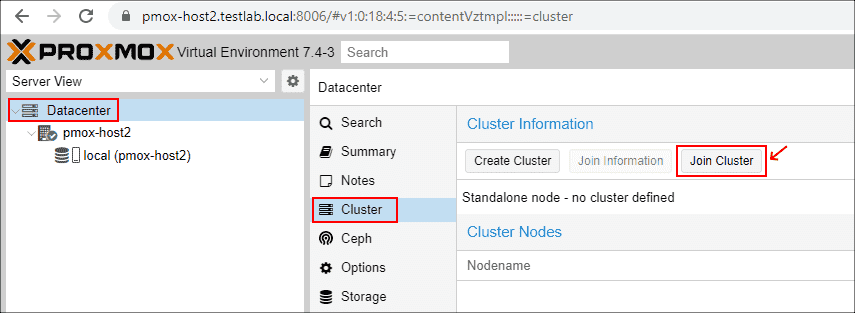
\includegraphics[width=0.75\linewidth]{"Pics/join-cluster.png"}
				\caption{Tạo và gia nhập các máy chủ thành với cluster}
				\label{fig:logo-hvMo_hinh_cong_ty}
			\end{figure}
			
			\hspace{0.3cm}{Sau khi gia nhập các máy chủ thành cluster thành công, chúng ta bắt đầu tạo ra một nơi lưu trữ chính cho cluster. Ở đây, công ty đã yêu cầu triển khai hệ thống quản lý dung lượng Ceph Storage.\\}
			
			\hspace{0.3cm}{Ceph Storage là một giải pháp quản lý dung lượng, phần mềm này được phát triển và sử dụng bởi nhiều mô hình trên thế giới ví dụ như AWS,... Ceph cung cấp cho khả năng tạo các ổ đĩa ảo được đính kèm vào các máy ảo, qua đấy các ổ được lưu trự và quản lý bởi Ceph.\\}
			
			\hspace{0.3cm}{Với Ceph Storage, có 3 máy chủ được phân cho sử dụng Ceph Storage Cluster. 3 máy chủ sẽ được cài hệ điều hành là Debian. Tương tự như việc cài đặt hệ điều hành Proxmox, em sử dụng các USB được cấp bởi công ty, cài đặt cho server hệ điều hành Debian. Sau khi cài đặt xong hệ điều hành, em sẽ tiến hành cài đặt Ceph Storage trên máy chủ. Ceph Storage cần cài đặt các thành phần như docker, cephadm. Sau khi cài xong, sử dụng các câu lệnh khởi tạo từ cephadm để tiến hành tạo ra master cho cluster. Cùng với đó, 2 máy chủ còn lại sẽ được lấy các thông tin như IP, user để cho ceph master tiến hành ssh vào các máy còn lại và liên kết chúng thành một cụm cluster.\\}
			
			\hspace{0.3cm}{Proxmox có tính năng tích hợp với Ceph Storage, vì vậy Ceph Storage sẽ được sử dụng cho việc cung cấp các ổ đĩa cho các máy ảo tạo ra bởi Proxmox. Bản thân Proxmox cũng có tính năng tạo ra Ceph Storage giữa các node khác nhau, tuy nhiên tính năng này có nhiều mặt hạn chế, và tính năng không được đầy đủ như Ceph Storage tự cài đặt bên ngoài. Vì vậy nhóm em đã lựa chọn cài đặt Ceph Storage thành một cluster riêng thay vì bật trực tiếp trong Proxmox.}
			
			\hspace{0.3cm}{Sau khi tích hợp với Ceph Storage, em sẽ tiến hành upload các base ISO của các hệ điều hành như Ubuntu, Debian, Windows Server,... vào một phân vùng được tạo ra từ Ceph. Các máy ảo sẽ được tạo ra từ các base ISO này. Trước hết, em sẽ tiến hành khởi tạo các máy ảo từ các ISO đã tải lên, và tiến hành tạo ra các template để giúp cho việc khởi tạo máy chủ nhanh hơn về sau này.\\}
			
			\hspace{0.3cm}{Template là tính năng đóng gói các máy ảo được tạo ra trong Proxmox, các máy ảo này sẽ được lưu giữ trạng thái cuối cùng khi tắt, sau đấy sẽ được đóng gói lại. Các template này sẽ được dùng khi cần, nhằm mục đích tiết kiệm thời gian khởi tạo các máy ảo. Việc template các máy ảo ban đầu sẽ mất kha khá thời gian, tuy nhiên, khi đã có template của các máy chủ, thì việc khởi tạo ra một máy ảo trong Proxmox sẽ diễn ra rất nhanh chóng.}
			
		\subsection{Bàn giao sản phẩm}
			\hspace{1.0cm}{Sau khi hoàn thiện sản phẩm, công ty đã bắt đầu ứng dụng sản phẩm vào các dự án đã và đang hoạt động. Sản phẩm đã hoành thành được các nhiệm vụ như triển khai các server nhanh chóng cho dự án, tạo dựng môi trường biệt lập cho dự án.\\}
			
			\hspace{0.3cm}{Quá trình yêu cầu sử dụng sản phẩm, đã được công ty đưa vào các quy tắc chung để giúp cho dự án mới có thể dễ dàng làm những phiếu yêu cầu sử dụng một cách nhanh chóng, thuận tiện.}
		\section*{Kết luận}
			\hspace{1.0cm}{Qua các phần trên, đó là những công việc mà em đã làm trong khi tham gia thực tập tại DUBE Technology. Những công việc này giúp em có cái nhìn sâu hơn về hệ thống, cách thức hoạt động cũng như cách thức triển khai một hệ thống cho công ty, doanh nghiệp. Công ty cũng đã giúp em rất nhiều trong những việc tìm hiểu, triển khai cũng như giúp đỡ em trong các khó khăn mà em gặp phải do kinh nghiệm còn thiếu xót.\\}
			
			\hspace{0.3cm}{Được sự giúp đỡ từ công ty, cũng như những đàn anh, đàn chị trong công ty, em đã có thể thành công phát triển, triển khai một hệ thống đầu tiên cho công ty cũng như có một dấu ấn về kiến thức nhất định của em trong con đường sự nghiệp phía trước.\\}
			
			
			
\end{document}